

\section{Examples%
  \label{examples}%
}

The purpose of the ScopeSim ecosystem is to simulate data from astronomical instruments.
As the saying goes: Pictures are worth a thousand words.
This section will illustrate how this is done with very few lines of python code for three common science cases.
It is the authors' hope that the code snippets provided are readable by the audience of this paper.
It this is in fact not the case, the authors refer the reader to the scopesim online documentation.


\subsection{Example 1: Extended source imaging%
  \label{example-1-extended-source-imaging}%
}

\begin{figure}
\noindent\makebox[\linewidth][c]{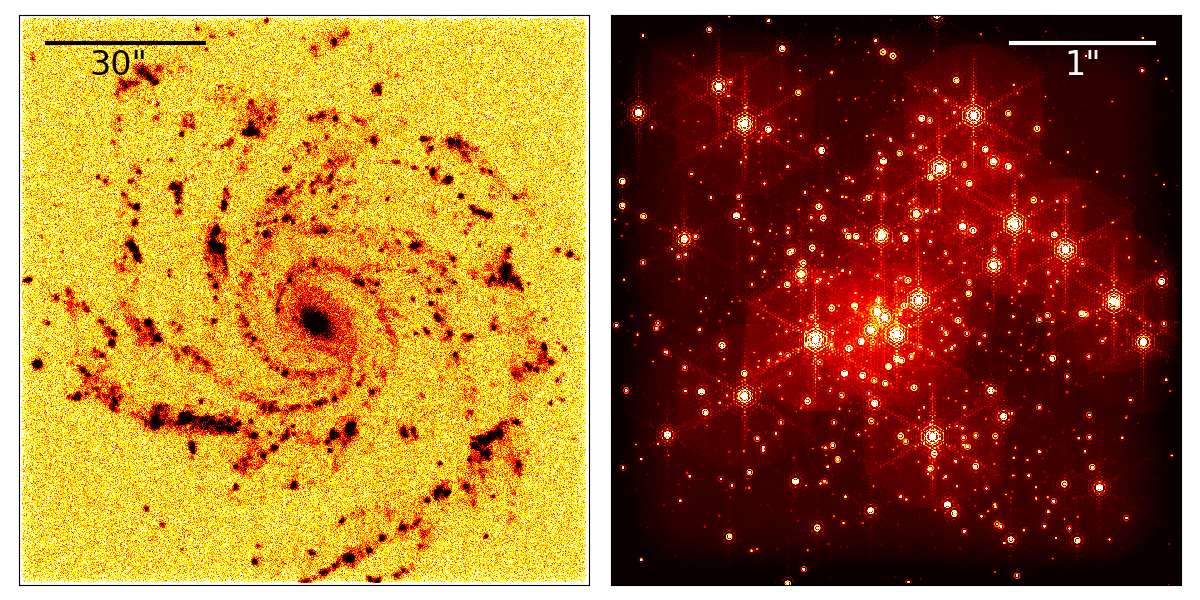
\includegraphics[scale=0.900000]{combined_1_2.png}}\phantomsection\label{fig-combined-1-2}

\caption{Left: A simulated one second observation in the Ks filter of a spiral galaxy similar to NGC,1232L using HAWKI at the VLT
Right: A simulated one hour observation in the Ks filter of a dense 3000,M\$\_odot\$ star cluster in the Large Magellanic Cloud using MICADO at the ELT.}
\end{figure}

The first short example simulates a short (1 second) exposure with HAWKI \citep{hawki} at the VLT in No-AO mode using the Ks filter.
The target is a two component spiral galaxy using a template based on NGC,1232L from the scopesim\_templates package.
The galaxy was resized to a diameter of 3 arcminutes and the associated flux spectra from \citet{brown2014} were rescaled to \textasciitilde{}12,mag,arcsec\$\textasciicircum{}\{-2}\$.
The detector window of 1024,\$times\$,1024 pixels covers \$sim\$1.6,\$times\$,1.6,arcminutes on sky.
The final simulated image shows primarily the star forming regions in the inner regions of the spiral arms.
The simulated detector output is shown in the left panel of Figure \ref{fig-combined\_1\_2}.

This simulation setup was chosen to illustrate the noise characterises introduced by ScopeSim.
The observation simulation requires only the following 8 lines of code:

\begin{quote}
\begin{alltt}
\begin{lstlisting}[frame=single]
import scopesim
from scopesim_templates.basic.galaxy import spiral_two_component

scopesim.download_packages(["locations/Paranal",
                            "telescopes/VLT",
                            "instruments/HAWKI"])

spiral = spiral_two_component(extent=180,       # arcsec
                              fluxes=(15, 12))  # mag

hawki = scopesim.OpticalTrain("HAWKI")
hawki.cmds["!OBS.dit"] = 1                      # seconds
hawki.observe(spiral)
fits_hdulists = hawki.readout()
\end{lstlisting}
\end{alltt}
\end{quote}

The simulation work flow will be discussed in more detail later in this paper.
Briefly it involves downloading the instrument packages relevant to the observation, generating an on-sky source target, creating a model of the combined optical system, and observing and reading out the detectors in the instrument model.
The output is a FITS HDUList, containing the instrument data in the format generated by the instrument.
By default the HAWKI package produces 1024,\$times\$,1024 images from a fictional detector window located at the centre of the focal plane.
The package however also includes the configuration data needed to produce the standard 2,\$times\$,2 grid of 2048,\$times\$,2048 detector images.
Switching between the two configuration is a simple matter of turning off the fictional detector window and turning on the realistic representation of the real detector array.


\subsection{Example 2: Point source imaging%
  \label{example-2-point-source-imaging}%
}

The major structures seen in the galaxy image produces in Example 1 are star forming regions.
Given the pixel-scale of HAWKI (0.106\textquotedbl{},pixel\$\textasciicircum{}\{-1}\$) it would be impossible to resolve the individual stars in these regions.
MICADO on the ELT, with its 4,mas,pix-1 pixel-scale (micado) and adaptive optics (AO) capabilities may well be able to detect individual stars in these regions.

The following code shows how to use the ELT and MICADO (Science Team) packages to simulate observations of highly dense star cluster outside the Milky Way.
The result of this code is show in the right panel of Figure \ref{fig-combined-1-2}:

\begin{quote}
\begin{alltt}
\begin{lstlisting}[frame=single]
import scopesim
from scopesim_templates.basic.stars import cluster

scopesim.download_packages(["locations/Armazones",
                            "telescopes/ELT",
                            "instruments/MICADO_Sci"])

cluster = cluster(mass=3e3,                     # solar masses
                  distance=50e3,                # parsec
                  core_radius=0.3)              # parsec
micado = scopesim.OpticalTrain("MICADO_Sci")
micado.cmds["!OBS.dit"] = 3600                  # seconds
micado.observe(cluster)
fits_hdulists = micado.readout()
\end{lstlisting}
\end{alltt}
\end{quote}

This code uses the star cluster template from the scopesim\_templates package to create a model of a dense star cluster located in the Large Magellanic cloud (D\textasciitilde{}50kpc), with a core radius of 0.3pc and a mass of 3000 Msun.
An exposure time of 1 hour with the Ks filter was used for the simulated observation.
This setup was chosen to show the effect of the ELT PSF on observations of densely populated fields with several bright sources.

It should be noted that the instrument package used above (MICADO\_Sci) is the slimmed down version of the full MICADO instrument package.
Simulations using the MICADO\_Sci package are less computationally intensive than when using the full MICADO package (which is aimed at pipeline development).
The MICADO\_Sci package was compiled specifically for the MICADO science team to test the feasibility of various science cases with MICADO and the ELT.


\subsection{Example 3: Spectroscopy%
  \label{example-3-spectroscopy}%
}

\begin{figure}
\noindent\makebox[\linewidth][c]{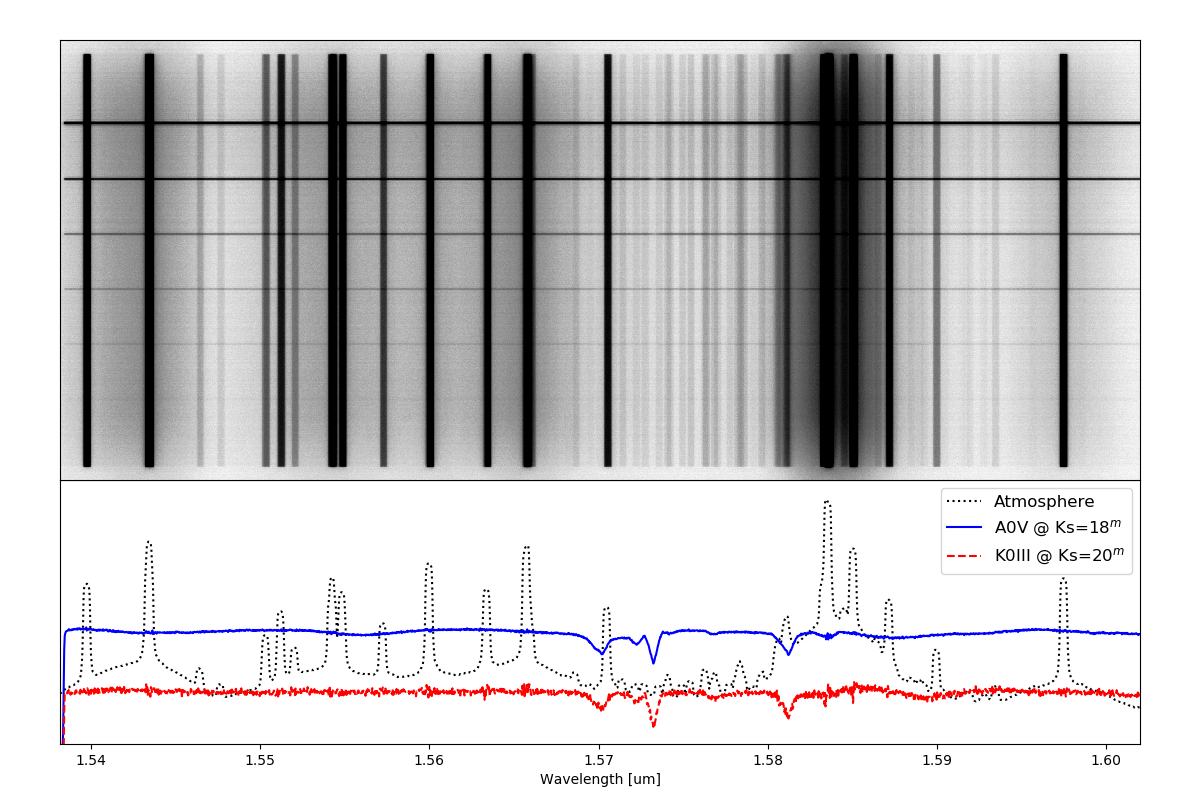
\includegraphics[scale=0.900000]{example_3_spectra.png}}\phantomsection\label{fig-example-3-spectra}

\caption{Top: A rectified spectral image from the MICADO detectors for a 1 hour spectrographic observation of 6 progressively fainter stars (18<=Ks<=23)
The dark vertical bars are the atmospheric emission lines.
The thin horizontal bars are the observed stellar spectra.
The simulated wavelength range was restricted to \$1.54<lambda<1.6mu m\$
Bottom: Extracted spectra for the brightest (Ks=18\$\textasciicircum{}m\$), third brightest (Ks=20\$\textasciicircum{}m\$) stars, and the atmospheric background.
The atmospheric background sprectum has been subtracted from the stellar spectra.
The noise in the fainter stellar spectrum is a result of the simulated noise characteristics introduced by ScopeSim.}
\end{figure}

The third example illustrates that ScopeSim can also be used to simulate spectroscopic observations.
While MICADO is primarily a near infrared imaging camera, it will also contain a long-slit spectrograph.
The spectroscopic mode of the MICADO\_Sci package allows the user to simulate reduced spectral trace data over a restricted wavelength range data - similar to what can be expected as output from the MICADO data reduction pipeline.

The following code simulates the spectral traces of 6 stars spaced equidistantly along the long-slit aperture with magnitudes in the range Ks={[}18, 23{]}.
In order to reduce computation time, the simulated wavelength range is restricted to 1024 spectral bins either side of a desired wavelength (1.578um).

\phantomsection\label{code-example-3-spectra}
\begin{DUclass}{code}
\begin{quote}
\begin{alltt}
\begin{lstlisting}[frame=single]
import numpy as np
from scopesim import UserCommands, OpticalTrain
from scopesim_templates.basic.stars import stars

stars = stars(filter_name="Ks",
              amplitudes=np.linspace(18, 23, 6)*u.mag,
              spec_types=["A0V", "G2V", "K0III"]*2,
              x=np.linspace(-1, 1, 6),
              y=[0]*6)
cmds = UserCommands(use_instrument="MICADO_Sci",
                    set_modes=["SCAO", "SPEC"],
                    properties=\{"!OBS.dit": 3600,
                                "!SIM.spectral.wave_mid": 1.578,
                                "!SIM.spectral.spectral_resolution": 0.00001,
                                "!DET.height": 2048,
                                "!DET.width": 800})
micado_spec = OpticalTrain(cmds)
micado_spec.observe(stars)
micado_spec.readout(filename="basic_spectral_trace.fits")
\end{lstlisting}
\end{alltt}
\end{quote}
\end{DUclass}

As can be seen in Figure \ref{fig-example-3-spectra} the atmospheric emission lines are prominent in the simulated raw detector output.
The 6 stellar spectra can be seen as thin horizontal lines.
The spectra displayed in the lower panel of Figure \ref{fig-example-3-spectra} were extracted for the detector readout in the upper panel.
The noise in the (red) K0III spectrum is a product of the noise characteristic of the simulated observation.
These include, but are not limited to photon shot noise and electronic noise sources.


\subsection{Effects included in instrument packages%
  \label{effects-included-in-instrument-packages}%
}

The instrument packages used for these examples can be found online in the Instrument Reference Database (IRDB) Github repository (see Section \ref{sec-docs-and-code}).
Each package contains a description of the optical effects that are inherent to the instrument or telescope, as well as the data needed to replicate these effects.
ScopeSim allows the user to view which effects are included in the current optical model.
This example uses the MICADO\_Sci optical system from the previous examples:

\begin{quote}
\begin{alltt}
\begin{lstlisting}[frame=single]
micado = scopesim.OpticalTrain("MICADO_Sci")
print(micado.effects)
\end{lstlisting}
\end{alltt}
\end{quote}

During run-time ScopeSim creates an Effect object for each effect listed in the instrument configuration files.
It then applies each of these Effect objects to the on-sky Source description in turn.
Effects can be included or excluded from a simulation by using the \textquotedbl{}.include\textquotedbl{} flag on the relevant Effect object:

\begin{quote}
\begin{alltt}
\begin{lstlisting}[frame=single]
micado["readout_noise"].include = False
micado["shot_noise"].include = True
\end{lstlisting}
\end{alltt}
\end{quote}

More information about the Effect objects is given in Section \ref{sec-architecture} as well as in the online documentation.
